\section{Casi d'Uso}

%	Vengono qui descritti:
%	1subs. I vari casi d'uso funzione delle specifiche richieste per l'API
%	2subs. I vari casi d'uso con estensioni di una eventuale applicazione di persistenza all'API

	\subsection{API}

	La realizzazione dell'API, \textit{Application Programming Interface}, è da contestualizzarsi all'interno dell'attività progettuale di tirocinio, svolta assieme al collega Gianmaria Del Monte. Il sistema preso qui in esame, è uno studio e realizzazione di protocollo efficiente per l'integrità dei dati su Cloud nell'ambito di un progetto di ricerca(6) del professor Maurizio Pizzonia, svolto a più livelli di astrazione. Si richiama qui la parte svolta dal collega, di cui sul suo scritto(7) è operata una descrizione più dettagliata, con lo scopo di definire casi d'uso e requisiti necessari.
	
	Il contesto, in breve, prevede un numero variabile di \textit{client}, con una disponibilità limitata in termini di memorizzazione, \textit{storage}, ma che necessita di salvare una grande mole di dati. Questo sarà reso possibile da un \textit{server}, considerata parte non fidata, il cui compito comprenderebbe anche l'attuazione del protocollo, delegando a particolari client, detti \textit{autenticatori}, il compito di autenticare le richieste provenienti dai client. Questi ultimi provvederanno all'autenticazione tramite firme, con una criptazione asimmetrica, verificabili tramite dei \textit{certificati}, noti a tutti i client. L'autenticazione di un valore relativo ad una richiesta di un client, tuttavia, dipenderebbe dall'avvenuta firma delle richieste precedenti.
	La forza del protocollo sta nella possibilità di attuazione di una architettura parallela di \textit{autenticatori}, i quali sarebbero in grado di autenticare un valore $ r_{i} $, anche se il valore precedente $ r_{i-1} $ non è ancora stato firmato. Dunque intuitivamente, l'autenticazione può avvenire in maniera \textit{condizionata} rispetto alla \textit{catena} di valori precedenti, permettendo al server di richiedere una autenticazione quando la precedente non è ancora finita.
	
	\begin{figure}
		\centering
		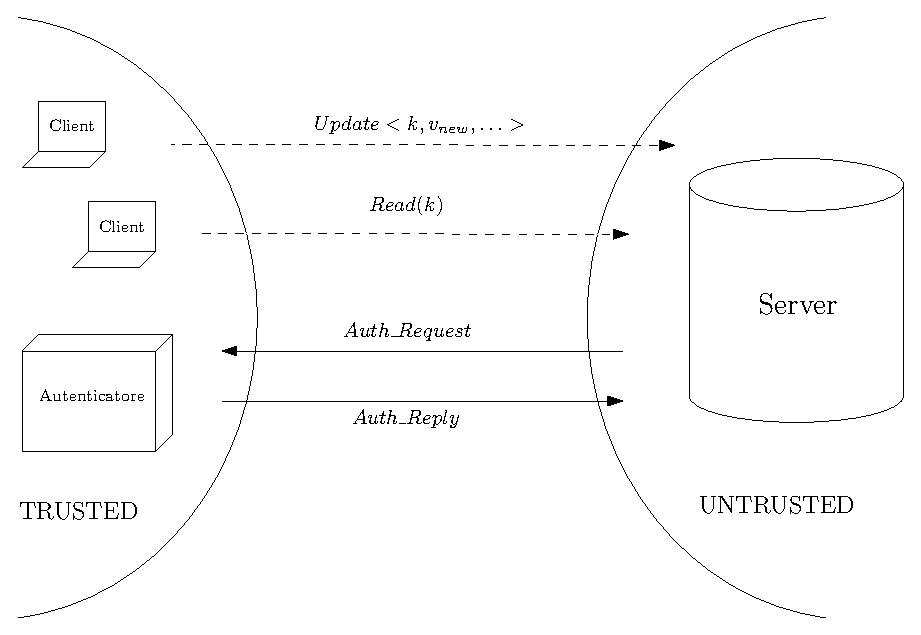
\includegraphics[scale=0.6]{figure/semicircles.eps}
		\caption{Il server riceve e accumula un certo numero di updates e richiede poi l'autenticazione tramite una authentication request, riceverà poi una authentication reply non appena sarà avvenuta l'autenticazione}\label{fig:semicircles}
	\end{figure}
	
	Fatte queste premesse, di seguito si elencano i casi d'uso della libreria(7):
	
	\begin{itemize}
		\item Una struttura dati autenticata, impostata come \textit{key-value store}, in grado di fornire operazioni di lettura e di scrittura, per ADSManager
		\item Una forma di prova di validità, nel seguito \textit{Proof}, per una o più chiavi presenti nella struttura
		\item Possibilità di ottenere dalla struttura dati autenticata il \textit{digest}, nel seguito \textit{root Hash}, relativo a tutte le coppie chiave-valore presenti
		\item Possibilità di ottenere dalla \textit{Proof}, il \textit{root Hash} relativo alla chiave o all'insieme di chiavi sulle quali è costruita, per ProofVerifier
		\item Capacità della \textit{Proof} di aggiornarsi rispetto agli update che avvengono sulla struttura dati autenticata principale, per poter fornire il \textit{root Hash} aggiornato, per RootHashCalculator.
 		\item Una struttura dati autenticata in grado di effettuare una serie di update, e in grado di restituire una \textit{Proof} cumulativa per questi update.
	\end{itemize}
	
	Oltre a i requisiti funzionali di cui sopra, altre specifiche di cui si è tenuto conto riguardano aspetti di \textit{usabilità}, nel fornire un'interfaccia di chiara e facile interpretazione ai fini dell'utilizzo dell'API, di \textit{prestazioni}, al fine di mirare al curve fitting con la complessità logaritmica, e di \textit{sostenibilità}, per garantire alta manutenibilità, verificabilità e configurabilità della API.
	
	Infine è doveroso menzionare i vincoli di progetto:
	\begin{itemize}
		\item Compatibilità della libreria con utilizzo concorrente.
		\item Utilizzo della Skip List come struttura di base per realizzare l'ADS.
		\item Linguaggio di programmazione JVM-Oriented.
	\end{itemize}

	\subsection{Persistenza}
	
	Per quanto riguarda la seconda parte, questa è da interpretarsi come una estensione delle API, atta a fornire la possibilità di memorizzare la struttura dati autenticata in persistenza, continuando ad ottemperare ai requisiti sopra esposti. Uno tra i principi cardine di questo studio consiste nel garantire la trasparenza dell'API rispetto a questa estensione. Pertanto essa non avrà bisogno di essere modificata a seguito dell'introduzione delle modifiche per la persistenza. Ovviamente il servizio dovrà essere affidabile, sempre attivo e dovrà avere la capacità di tollerare guasti, errori e fallimenti.
	Oltre a questo, l'obiettivo principale, per cui nei successivi capitoli è presente un'approfondito studio teorico, è quello dell'efficienza, cercando di operare caricamenti e query in maniera parallela piuttosto che sequenziale.
	Anche per questa sezione è presente un vincolo di progetto, che riguarda l'interoperabilità con un database management system di tipo non relazionale.

\section{Modello di Dominio}

%	In base ai casi d'uso e, in qualche modo, ai requisiti sopra citati viene illustrato un analogo di modello di dominio.
	
 	Si procede, dunque, in questa sezione, dipendentemente dai casi d'uso e dai requisiti funzionali e non, sopra esposti, all'enumerazione dei concetti significativi nell'ambito di un modello di dominio. I concetti qui esposti, saranno poi più dettagliatamente spiegati nei successivi paragrafi, ma sono qui anticipati con lo scopo di fornire una rappresentazione visuale di entità concettuali rilevanti.
 	Ebbene, sicuramente sarà necessaria un'entità che rappresenti la struttura dati autenticata, la quale dovrà essere in grado di offrire servizi di lettura e scrittura, rispettivamente di query e update. Essa inoltre deve essere in grado di fornire le \textit{Proof} necessarie ai client o agli autenticatori per effettuare le prove di integrità dei dati. Allo stesso tempo la \textit{Proof} deve saper fornire il \textit{root Hash} relativo alle chiavi sulle quali è definita, e deve saper applicare degli update sulle suddette chiavi. Inoltre, intuitivamente, sarà necessario che due \textit{Proof} per due diversi insiemi di chiavi, possano unirsi, tramite un \textit{merge} dando vita ad una \textit{Proof} valida per entrambi gli insieme di chiavi di partenza.

	
\section{Skiplist}

%	In questa parte si parla della struttura dati utilizzata, studiata e realizzata. Ricordando che siamo all'interno della parte di analisi
%	è interessante richiamare a precedenti contestualizzazioni ed eventualmente fornire una generale descrizione della struttura che 
%	sia in grado di dare un'idea. Eventualmente fare analogia con alberi.
%
%	{Immagini}

	Prima di entrare nel dettaglio dell'analisi riguardante le strutture dati autenticate, si ritiene necessaria una preliminare analisi della struttura che sta alla base di tutto ciò: la skip list. In letteratura frequente è la scelta di strutture dati come alberi binari di ricerca bilanciati: si pensi agli alberi rosso-neri, una tra le più utilizzate implementazioni.
	
	La scelta di adozione di questa particolare struttura, sebbene risulti vincolo di progetto, rispecchia molte necessità richieste dall'utilizzatore. Di seguito se ne presentano le principali.
	
	La skiplist risulta essere più gestibile e adatta per quanto riguarda accessi e/o modifiche concorrenti. Infatti nel caso degli alberi rosso-neri il problema sussiste dal momento in cui le operazioni di modifica comportano sempre la necessità di bilanciamento della struttura. Questa operazione può interessare anche gran parte della struttura stessa, risultando talvolta anche largamente bloccante per altre eventuali operazioni effettuate in ambito concorrente. Altri utenti infatti, potrebbero voler accedere, in scrittura o in lettura, a nodi che devono ancora essere processati. Le performance di un albero rosso-nero, come detto una delle principali implementazioni di alberi di binari di ricerca, risulterebbero degradare linearmente per ogni nuovo utente concorrente. Realizzazioni più rigide di questa struttura comportano infatti lo stato bloccante su tutti i nodi della struttura durante il bilanciamento, e, nonostante esistano realizzazioni più rilassate, queste non hanno un impatto rilevante nel miglioramento delle performance (1)
	Letture e scritture in una skiplist risultano invece molto più localizzate e solo pochi nodi, quelli direttamente interessati, richiedono lo stato bloccante.
	
	La skip list, dunque, soddisfa la contemporanea necessità di avere una struttura dati ordinata e che sia thread-safe, cioè adatta ad un contesto concorrente.
	
	E' inoltre opportuno precisare da un lato il maggiore spazio richiesto dalle skiplist rispetto ad alberi bilanciati, in quanto necessitano, in media, del doppio dei puntatori per nodo, e dall'altro però la loro estrema facilita di implementazione.
	
	\subsection{Definizione}
	
%		Qui si procede con una più precisa e dettagliata definizione della struttura
%		
%		{dimostrazioni MIT}
%		{Immagini}

	Dopo averne brevemente motivato l'adozione, si procede con una più precisa definizione che possa aiutare il lettore a comprendere appieno il razionale retrostante questa struttura. 
	La skip list è una struttura dati probabilistica che permette veloci ricerche all'interno di una sequenza ordinata di elementi. Essa mantiene un insieme ordinato di $ n $ elementi in tempo $\mathcal{O}(log{}n)$.
	
	Prendendo ad esempio una lista semplice e non ordinata di elementi, si noti che l'operazione di ricerca di un elemento venga soddisfatta in tempo $\mathcal{O}(n)$. Questo vale anche per una lista ordinata di elementi. Questo tuttavia è vero nell'ipotesi in cui sia possibile accedere alla lista solamente tramite un puntatore verso l'inizio della stessa. Nell'ipotesi invece di accesso randomico a qualsiasi elemento, è possibile effettuare un'operazione di ricerca in tempo $\mathcal{O}(log{}n)$. Ebbene questa è l'idea retrostante.
	Tutto questo è reso possibile grazie ad una gerarchia di sottosequenze, organizzate su più livelli collegati tra loro. Lo sviluppo è in altezza e prevede che il livello più basso, detto \textit{base list} contenga tutti gli $ n $ elementi, mentre ogni livello superiore è composto da un sottoinsieme degli elementi del livello immediatamente sottostante. Le operazioni di ricerca iniziano dal livello con meno elementi, ovvero quello all'apice della struttura, e procedono per salti, in gergo 'skip', di nodo in nodo, fino a che non vengono trovati due elementi consecutivi, uno minore e uno maggiore o uguale all'elemento ricercato. A questo punto, grazie ai collegamenti inter-livello è possibile spostarsi sulla sottosequenza immediatamente inferiore e proseguire la ricerca. Questo procedimento è ripetuto fino a giungere alla sequenza completa di elementi, ovvero al livello più basso.
	Ogni livello inoltre, agli estremi, possiede due sentinelle, ovvero due nodi speciali, marcati con $\infty$ e -$\infty$. Questi formeranno due torri, che racchiudono a destra e a sinistra la struttura contenente gli elementi veri e propri. Si può dimostrare però che ciò non è sempre completamente necessario, ma si tratta più di rigorosità nella formulazione.
	Il nodo sentinella -$\infty$ della sequenza all'apice della struttura è detto \textit{start node} ed è il nodo di partenza per ogni operazione.
	
	Il principio secondo cui gli elementi sono saltati, e quindi indirettamente il principio secondo cui un elemento debba o meno essere presente anche nel livello immediatamente superiore, può essere randomico o deterministico. Il primo caso, di più frequente utilizzo, prevede una costruzione della struttura per strati. Il primo, contenente tutti gli $ n $ elementi è una normale lista doppiamente o singolarmente concatenata. Ogni livello superiore poi è costruito a partire da quello sottostante, dove però ogni elemento ha una certa probabilità, fissata a priori, di essere presente. Normalmente la probabilità fissata a priori è $ 1/2 $, a tal punto che in letteratura si parli spesso di 'Fair coin flip'.
	
	Prima di procedere con la descrizione dettagliata delle operazioni che fornisce, occorre introdurre ulteriore terminologia. Un nodo di un livello $ L_{i-1} $ contenente un elemento che non è presente al livello $ L_{i} $ è detto \textit{plateau}. Un nodo che non presenta queste caratteristiche è detto \textit{tower}. (2)
	
	Per comodità delle future analisi si è deciso di adottare una terminologia simile allo scritto di Goodrich e Tamassia (2), a cui ci si rifarà anceh nel successivo sottoparagrafo, in cui per ogni nodo $ v $ della sottosequenza $ L_{i} $, è detto $ elem(v) $ l'elemento memorizzato in $ v $. Inoltre è detto $ down(v) $ il nodo della sottosequenza $ L_{i-1} $ che memorizza lo stesso valore di $ v $, a meno che non si tratti della \textit{base list}, poiché in questo caso $ down(v) = \boldmath{null}$.
	Inoltre è detto $ right(v)$ il nodo della sottosequenza $ L_{i} $ immediatamente alla destra di $ v $, a meno che non si tratti di una sentinella di tipo $\infty$, per la quale $ right(v) = \boldmath{null}$.
		
	\begin{figure}
		\centering
		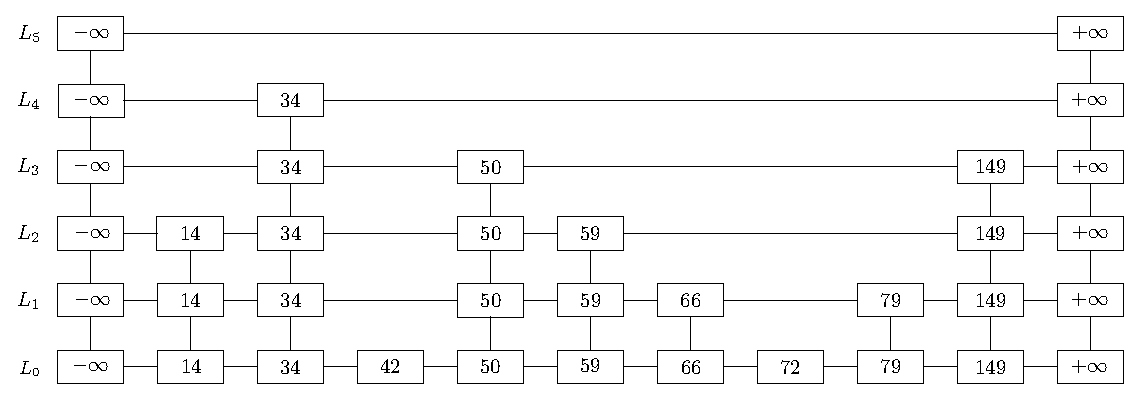
\includegraphics[scale=0.6]{figure/skiplist.eps}
		\caption{Esempio di una Skip List}\label{fig:skiplist}
	\end{figure}
		
	\subsection{Operazioni principali}
	
%		Rimanendo sullo stesso livello di dettaglio raggiunto dalla sottosezione di definizione, si prosegue con una dettagliata analisi
%		delle principali operazioni operabili su una skiplist. Trovandoci nella parte di analisi si evidenzi il collegamento tra le parti: qui la
%		funzione di questa sezione è di introdurre alla struttura di base, che sarà poi ampliata e utilizzata nei paragrafi successivi quando
%		si aggiungerà l'autenticazione.
%		
%		Potrebbero essere utili immagini e pseudocodice, ma qui siamo ancora parlando della struttura di base pertanto si tratta di apporti
%		alquanto standard e non personali. Potrebbe dunque essere superfluo l'inserimento di pseudo. Le immagini potrebbero essere usate
%		per illustrare più intuitivamente i vari algoritmi che magari prima sono descritti molto più formalmente.
%		{Immagini}
%		{Pseudo}

		Dopo aver introdotto a grandi linee il razionale alla base della skip list, si procede in questa sezione ad una più dettagliata enumerazione delle operazioni che supporta:
		\begin{itemize} 
			\item \textbf{Ricerca}: determina se un elemento è o meno presente nella skip list.
			\item \textbf{Inserimento}: inserisce un elemento.
			\item \textbf{Cancellazione}: elimina un elemento.
		\end{itemize} 
	
		\subsubsection{Ricerca}
			
			L'operazione di ricerca di un elemento $ x $ in una skip list inizia, come tutte le altre, dallo \textit{start node}. La ricerca viene effettuata tramite l'alternanza di due azioni, \textit{hop forward} e \textit{drop down}, che rappresentano rispettivamente il movimento verso destra o verso il basso all'interno della struttura. Esse sono ripetute, sotto determinate condizioni, fino a che la ricerca non sia terminata, indipendentemente dall'esito, che potrà essere positivo o negativo.
			
			La prima azione menzionata prevede movimenti verso destra fino a che non si raggiunge un nodo il cui valore sia il più grande minore o uguale a $ x $. La seconda azione invece consiste semplicemente in uno spostamento verticale, al nodo immediatamente sottostante, a condizione che questo esista.  In pseudocodice, i passi rilevanti delle due azioni, rispettivamente: 
			
			\begin{itemize}
			
			\item \textbf{Hop forward}:
				\begin{algorithm}[H]
					\While{elem(right(v)) < x}{
						v $\leftarrow$ right(v)\;
					}
				\end{algorithm}
			
			\item \textbf{Drop down}:
				\begin{algorithm}[H]
					\eIf{down(v)  != null}{
						v $\leftarrow$ down(v)\;
					}{
						end search\;
					}
				\end{algorithm}
			\end{itemize} 
			
			La ricerca consiste dunque in un \textit{hop forward} e un \textit{drop down}, fintanto che risulti possibile effettuare \textit{dropdown}.  Con questa sequenza di passi si raggiungerà un nodo sulla \textit{base list}: se vale che $ elem(v) = x $ allora la skip list contiene l'elemento $ x $. Se questa condizione non risulta vera, allora il nodo raggiunto tramite questa sequenza di passi sarà il nodo sulla \textit{base list} con il valore più grande minore di $ x $. Per costruzione $ right(v) $ è il nodo sulla \textit{base list} il cui elemento è il più piccolo maggiore di $ x $.
			
			Il costo computazionale dell'operazione di ricerca è dato dalla somma dei costi di attraversamento di tutti i livelli. Tuttavia ogni livello, tranne il primo, subisce un attraversamento parziale, in quanto il nodo di partenza non è il primo nodo della sequenza.
			
			
			\begin{figure}
				\centering
				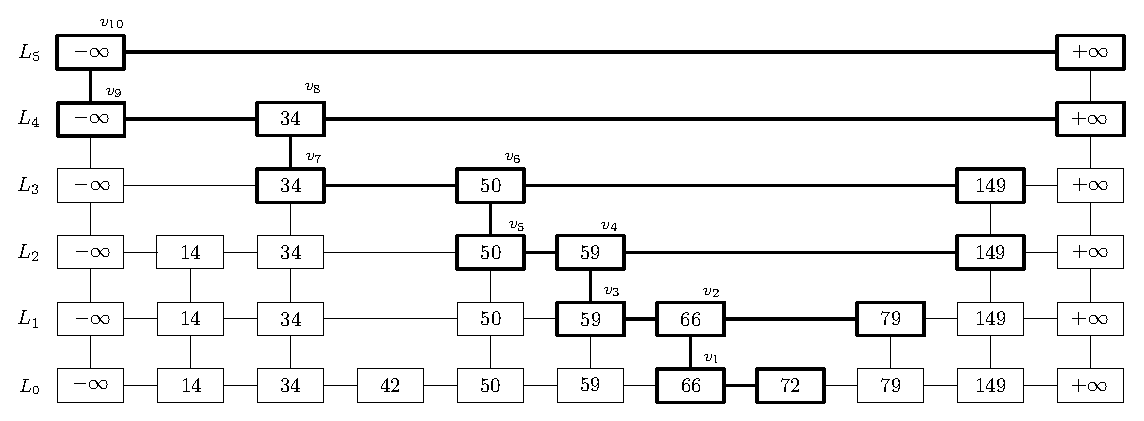
\includegraphics[scale=0.6]{figure/search-66.eps}
				\caption{\textbf{Ricerca dell'elemento 66} nella Skip List della figura \ref{fig:skiplist}. I nodi visitati e i collegamenti attraversati sono evidenziati con linee più spesse. Si noti che la ricerca, fallimentare, dell'elemento 70 produrrebbe lo stesso risultato.}\label{fig:2}
			\end{figure}
			
			{EVENTUALE DIMOSTRAZIONE MIT}
			
			Considerando che il numero di livelli in una skip list con $ n $ elementi è, con alta probabilità\footnote{Un evento occorre con alta probabilità quando la sua probabilità dipende da un certo valore $ n $ e tende a 1 quando $ n $ tende a $\infty$}, pari a $\mathcal{O}(log{}n)$, è dimostrabile che il costo di ricerca è, con alta probabilità, pari a $\mathcal{O}(log{}n)$.
				
		\subsubsection{Inserimento}
		
			L'operazione di inserimento è sempre preceduta da una operazione di ricerca. Dunque per inserire un elemento $ x $, per prima cosa è effettuata una ricerca su $ x $, con l'unica differenza che ogni volta che viene effettuato un \textit{hop forward} o un \textit{drop down} rispetto al nodo corrente $ v $, viene aggiunto un elemento in una pila che registri il nodo corrente $ v $ e l'azione associata.
			Dal momento in cui l'elemento $ x $ non è presente, l'operazione di ricerca restituirà il nodo sulla \textit{base list} che dovrà essere immediatamente precedente al nodo da inserire. Dunque è inserito il nodo, memorizzato il valore $ x $. Dopodiché, nel caso di skip list randomiche, viene valutata l'altezza della torre, ovvero in quali livelli superiori dovrà essere presente l'elemento, tramite una sequenza di tiri di moneta simulati. Per ogni lancio di moneta, nel caso in cui il risultato sia testa, viene utilizzato la pila per ripercorrere il percorso a ritroso e ottenere la posizione, del livello superiore, in cui dovrà andare il nuovo nodo, tramite opportune operazioni di \textit{pop}. Il procedimento continua fino a che il risultato non sia croce. Nel caso in cui la torre dovesse superare l'altezza corrente della struttura, si aggiunge un nuovo livello alla struttura, compresi ovviamente i nuovi nodi sentinella.
			L'operazione di inserimento è, con alta probabilità, pari a $\mathcal{O}(log{}n)$.
		
		\subsubsection{Cancellazione}
		
			L'operazione di cancellazione di un elemento $ x $ prevede la ricerca di un elemento che sia minore di $ x $ ma maggiore di ogni altro elemento nella \textit{base list} che sia minore di $ x $. Come per l'operazione di inserimento, viene utilizzata una pila di supporto per tenere traccia dei passi effettuati dalla ricerca. Chiaramente, l'elemento immediatamente successivo al nodo restituito dall'operazione di ricerca, dovrà essere $ x $, poiché in caso contrario l'elemento da cancellare non sarebbe presente nella skip list, scenario di non successo, da segnalare con errore opportunamente.
			Dunque viene rimosso il nodo interessato, e tutti i nodi sulla stessa torre, ottenendone la posizione grazie ad opportune operazioni di \textit{pop} dalla pila precedentemente riempita.
			Nel caso in cui la rimozione dovesse comportare un abbassamento globale della struttura, devono essere eliminati i nodi sentinella interessati.
			L'operazione di cancellazione è, con alta probabilità, pari a $\mathcal{O}(log{}n)$.
			
	
\section{Hashing Non-commutativo}
	
%	Qui si parla della tecnica di hashing commutativo

	Si ritiene necessario, a questo punto, introdurre una speciale classe di funzioni: le funzioni crittografiche di hash. Si tratta di algoritmi matematici che mappano, cioè fanno corrispondere, dati di lunghezza arbitraria, comunemente chiamati \textit{messaggi}, in un stringa binaria di dimensione fissa, detta \textit{valore di hash}. L'output prodotto è solitamente chiamato \textit{digest}. (4)
	L'hash di un messaggio $ m $ è denotato $ h(m) $ e varranno le seguenti proprietà:
	
	\begin{itemize}
		\item Per ogni $ m $ il calcolo di $ h(m) $ è efficiente;
		\item Dato un $ H $, è computazionalmente difficile trovare $ m $ tale che $ H = h(m) $;
		\item Dato $ h $, è computazionalmente difficile trovare un $ m \ne m^{'}$ tale che $ h(m) = h(m^{'}) $;
		\item Dato $ h $ e $ m $, è computazionalmente difficile trovare un $ m \ne m^{'} $, tale che $ h(m) = h(m^{'}) $. (5)
	\end{itemize}

	E' altrettanto vero che la funzione può essere applicata a due o più messaggi. Pertanto data una coppia di valori $ a $ e $ b $, sarà $ h(a,b) $ il digest prodotto dalla funzione di hash. Lo stesso è applicabile anche su triple, e più in generale su n-ple di lunghezza qualsiasi. Per effetture il digest di una sequenza $ (x_{1}, x_{2}, ... , x_{m}) $, dovrà essere effettuato il seguente calcolo: $ h(x_{1}, h(x_{2}, ... h(x_{m-2},h(x_{m-1},x_{m}))...)) $. (2)
	
		\subsection{Funzioni}
	
	%		Funzioni di hash, con eventuale breve richiamo alle loro differenze. Questo servirà a giustificare la resa parametrica
	%		nel codice e potrà servire ad introdurre la parte di analisi di prestazioni, nel caso di dettaglio dell'analisi computazionale
	%		(spazio e tempo) riguardo l'applicazione delle varie funzioni di hashing.
			
			Per lo scopo, possono essere adottati vari tipi di funzione di hash, sui singoli valori. Si è ritenuto importante garantire un certo livello di flessibilità, permettendo una scelta all'interno delle API. Le funzioni tra le quali è possibile scegliere appartengono a una famiglia delle funzioni crittografiche di hash, le \textit{Secure Hash Algorithms}, abbreviato \textit{SHA}. In particolare è possibile scegliere tra lo SHA-1, funzione di 160 bit la cui vulnerabilità crittografica è nota, lo SHA-256 e lo SHA-512, resistenti a pericolosi attacchi come il \textit{Length extension attack}, le quali differiscono nella dimensione della parola.
			
	\subsection{Resistenza a collisioni}
	
%		In questa sottosezione si approfondisce la caratteristica di resistenza a collisioni dell'hashing commutativo
%		con particolare attenzione all'utilità di questa caratteristica al nostro studio

		L'utilità di una funzione crittografica di hash all'interno di una struttura dati autenticata, di cui si parlerà più approfonditamente nel successivo paragrafo, è data dalla resistenza alle collisioni. Ovvero data una coppia di valori $ (a,b) $, risulta computazionalmente difficile trovare una coppia $ (c,d) \ne (a,b) $ tale per cui  $ h(a,b) = h(c,d) $. Infatti il costo computazionale richiesto per trovare una coppia di collisione $ (c,d) $ sarebbe troppo elevato anche per un supercomuter.
		La specifica di non commutatività della funzione di hash, serve a sottolineare l'esclusione della proprietà di commutatività che potrebbe essere inclusa per semplificare i processi di verifica effettuati dall'utente.
		In questo studio tuttavia essa non è permessa, causa vincoli di progetto, e dunque formalmente $ h(a,b) \ne h(b,a) $ per ogni $ a $ e $ b $.

	\subsection{Strutture dati autenticate}

% 		Introduzione su strutture dati autenticate. Magari breve, e mirata a far comprendere i sucessivi paragrafi

		Una struttura dati autenticata, abbreviato \textit{ADS}, è una struttura dati che è adatta a controlli sulla sua integrità, cosi come su porzioni di essa. Memorizza valori e associa una funzione crittografica di hash $ h $ con il suo contenuto. L'output prodotto da questa funzione è detto \textit{root hash} e possiede lunghezza finita. Tramite una ADS, dunque, un client può rilevare piccoli cambiamenti all'interno di un \textit{dataset} anche molto grande, in maniera efficiente.
		La sua applicazione in ambiente cloud risulta particolarmente proficua in quanto generalmente permette di ottenere elevate garanzie su sicurezza, autenticazione e verifica di integrità dei dati. Tutto questo rispettando la dicotomia tra l'ambiente di storage locale, limitato ma fidato, \textit{trusted}, e l'ambiente cloud, virtualmente illimitato, ma non fidato. Il razionale alla base consiste nel memorizzare un grande \textit{dataset} sul cloud, equipaggiato dunque con una ADS, e mantenere soltanto il root hash localmente.
		
		\begin{figure}
			\centering
			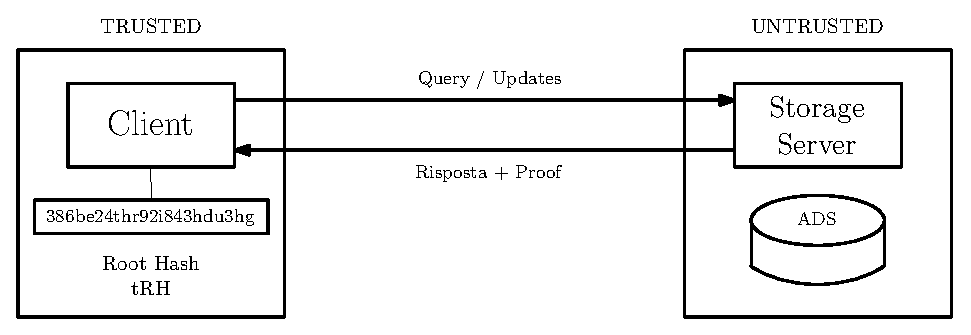
\includegraphics[scale=0.75]{figure/trusted-untrusted.eps}
			\caption{\textbf{Caso d'uso di ADS}: l'ADS può essere caricato sul cloud e applicato su uno \textit{storage} regolare, mentre il client memorizza localmente il Root Hash. Lo storage non dovrebbe essere a conoscenza dell'ADS.}\label{fig:3}
		\end{figure}
		
		\begin{itemize}
			\item Le varie query, effettuate dal client, restituiranno oltre ai valori richiesti, anche una prova, detta \textit{Proof}. Tramite la proof ricevuta e il root hash locale, il client potrà verificare l'integrità del risultato della query.
			
			\begin{figure}
				\centering
				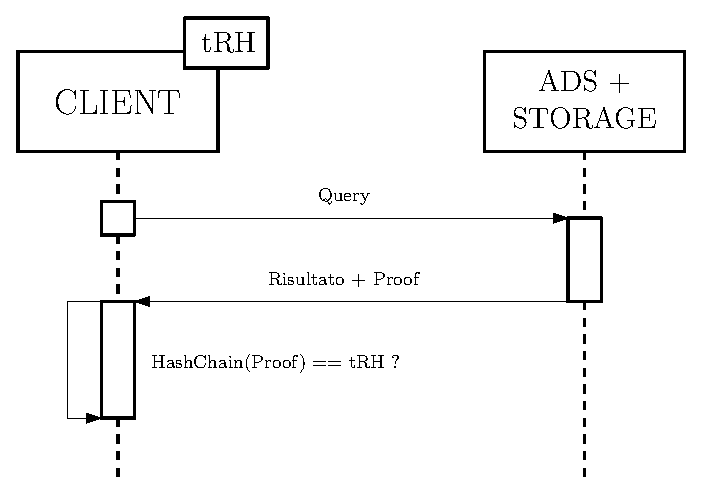
\includegraphics[scale=0.75]{figure/queryADS.eps}
				\caption{\textbf{Query}: il client effettua una query e riceve oltre al risultato atteso, una proof per quel risultato. Effettua dunque il calcolo localmente sulla proof e verifica se corrisponde al root hash locale.}\label{fig:4}
			\end{figure}
			
			\item Gli updates tuttavia, andranno a cambiare il \textit{dataset} remoto, e dunque l'ADS presente sul cloud. Il client inoltre aggiorna il suo root hash locale con quello nuovo prodotto dall'ADS.
			
			\begin{figure}
				\centering
				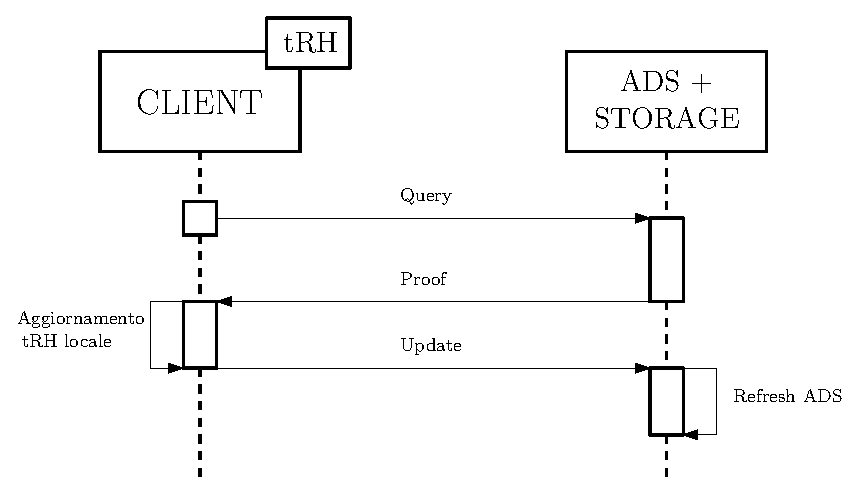
\includegraphics[scale=0.75]{figure/updateADS.eps}
				\caption{\textbf{Update}: il client richiede al server la proof su un valore da aggiornare. Può, a questo punto, aggiornare il root hash locale e inviare il nuovo valore al server. Suo è, successivamente, il compito di aggiornare l'ADS, \textit{refresh} in figura.}\label{fig:5}
			\end{figure}
		
		\end{itemize}
	
		Dunque, updates effettuati da un qualsiasi client, su un qualsiasi valore della struttura, si ripercuoteranno sul root hash della struttura, permettendo il rilevamento delle modifiche ad ogni altro client, in tutte le successive query.
		
		Le più diffuse implementazioni di strutture dati autenticate sono:
		
		\begin{itemize}
			\item Merkle Hash Tree (MHT);
			\item Skip list autenticate.
		\end{itemize}
	
		Il funzionamento di quest'ultima sarà approfondito nei successivi paragrafi.
	
\section{API}

%	{Analisi prettamente tecnologica}
%	
%	Qui, sulla base di quanto detto precedentemente, si inizia a mettere insieme le varie parti per descrivere più
%	nel dettaglio l'API. Già nella prima parte è stato introdotto a grandi linee il funzionamento. Qui viene ripreso e
%	approfondito, anche e sopratutto grazie alle sottosezioni successive. 

	Riallacciandomi a quanto detto nella sezione riguardante il modello di dominio, è possibile a questo punto aggiungere informazioni più precise. L'API girerà sul server, e dovrà consentire la gestione della simbiosi tra lo storage e appunto l'ADS. L'entità rappresentante la struttura dati autenticata, in base a vincoli di progetto, dovrà basarsi sulla Skip List. Si tratterà, dunque, di un \textit{key-value store} capace di offrire servizi di update e query, generando anche le opportune \textit{Proof} in base al particolare tipo di richiesta del client. L'elemento costituente della Skip List Autenticata, sarà un nodo, in grado sia di memorizzare la chiave relativa alla torre in cui si trova, sia gli hash dei nodi adiacenti. In questo modo la struttura potrà comportarsi come un'ADS a tutti gli effetti, in ottemperanza con i requisiti e con i casi d'uso. Il funzionamento preciso dell'API sarà affrontato con il dovuto dettaglio nella sezione di Progetto, mentre qui si vuole soprattutto spiegare il funzionamento concettuale e la collaborazione tra le parti.
	
	\begin{figure}
		\centering
		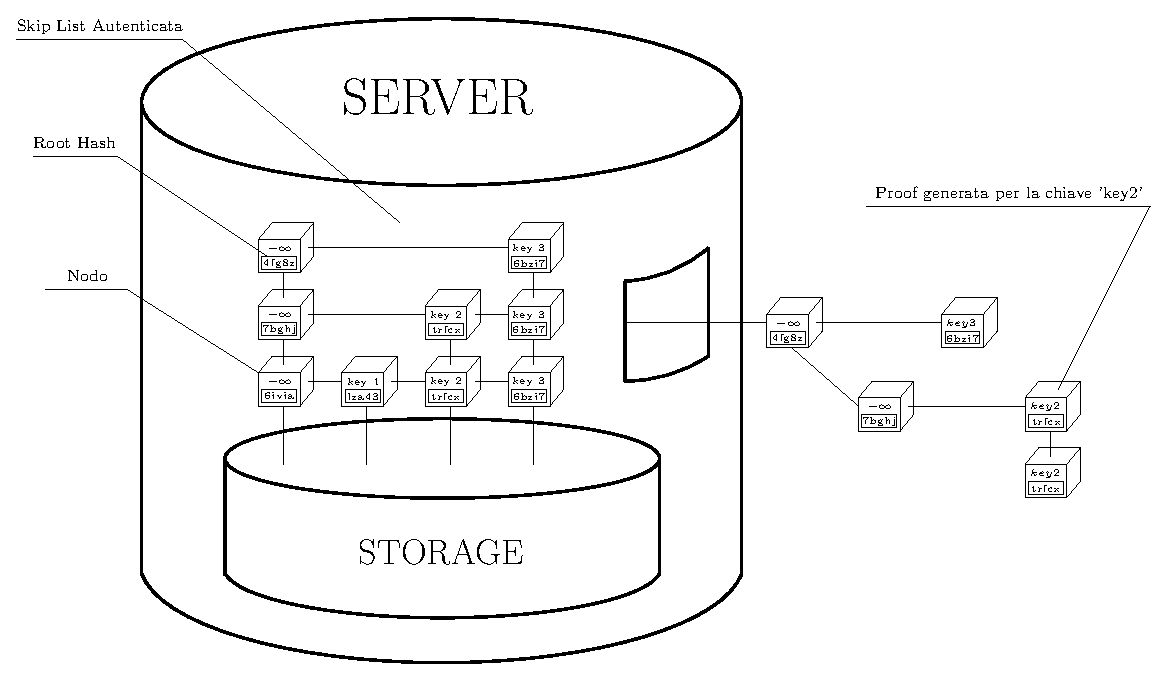
\includegraphics[scale=0.75]{figure/global.eps}
		\caption{In figura è rappresentata un'astrazione di ciò che è presente sul server, preso isolatamente. La Skip List Autenticata, il cui elemento base è il Nodo, sta "sopra" lo storage classico. Genera opportune \textit{Proof} in base alle richieste del client.}\label{fig:8}
	\end{figure}
	
	\subsection{Skip List Autenticata}
	
%		MODELLO FUNZIONALE, rimandando a parte successiva 
%		
%		Qui si parla della skiplist autenticata, facendo chiaramente riferimento alla skiplist base, sia nella definizione,
%		sia nella descrizione delle operazioni

	Una skip list autentiticata, come deducibile dalla figura \ref{fig:8}, è una particolare implementazione di un ADS, che si basa su skip list, e sulla quale è applicata una funzione crittografica di hash $ h $. La struttura dunque aggiungerà alla funzione di memorizzare un insieme di valori, in maniera ordinata, le caratteristiche tipiche di un ADS. Per permettere dunque sia l'ordinamento dei dati, sia l'applicazione di $ h $, si prende in esame una struttura  basata su coppie chiave-valore, entrambe di dimensione fissata a priori. In questo modo le chiavi permetteranno l'ordinamento dei dati, e i valori permetteranno l'applicazione dello schema di hashing, approfondito nel prossimo paragrafo. Ogni nodo conterrà, oltre alla chiave relativa alla torre su cui giace, un hash dei dati di alcuni altri nodi adiacenti. Intuitivamente, il suo hash potrebbe essere in funzione di $ w = right(v) $ e $ u = down(u) $. Questo schema confluirà nel root hash, ovvero nel \textit{digest} dell'intera skip list, il quale sarà memorizzato nello \textit{start node}.
	Il root hash, per definizione e per costruzione, sarà rigidamente dipendente sia dai valori di ogni nodo che dalla loro posizione reciproca. Da questo calcolo sono esclusi i nodi sentinella.
	
		\subsubsection{Schema hashing}
	
	%		In questa sottosezione ci si riallaccia alla sezione sull'Hashing non-commutativo e semplicemente
	%		si definisce la sua applicazione alla skiplist autenticata. Nella sezione sopra l'argomento è affrontato in maniera più
	%		teorica, preliminare, e isolata. Qui invece si sottolinea l'aspetto pratico sulla struttura dati.
	
		Il calcolo del root hash dunque è strettamente legato allo schema di hashing scelto, ovvero alla modalità secondo cui i singoli nodi calcolano il loro hash locale in funzione dei nodi adiacenti. Per questa analisi, si è deciso di seguire lo schema suggerito da Tamassia(2), con alcune piccole variazioni. 
		Sia $ f(v) $ la funzione di hash di ogni singolo nodo, allora varrà che:
		
		\begin{enumerate}
			\item Se $ u = null $, e cioè se il nodo $ v $ si trova sulla \textit{base list}:
				\begin{itemize}
					\item (a) Se $ w $ è un nodo \textit{tower}, allora $ f(v) = h(elem(v)) $.
					\item (b) Se $ w $ è un nodo \textit{plateau}, allora  $ f(v) = h(h(elem(v)), f(w)) $.
				\end{itemize}
			\item Se $ u \ne null $, e cioè se il nodo $ v $ \underline{non} si trova sulla \textit{base list}:
				\begin{itemize}
					\item (a) Se $ w $ è un nodo \textit{tower}, allora $ f(v) = f(u) $. 
					\item (b) Se $ w $ è un nodo \textit{plateau}, allora  $ f(v) = h(f(u), f(w)) $. 
				\end{itemize}
		\end{enumerate}
	
		\begin{figure}
			\centering
			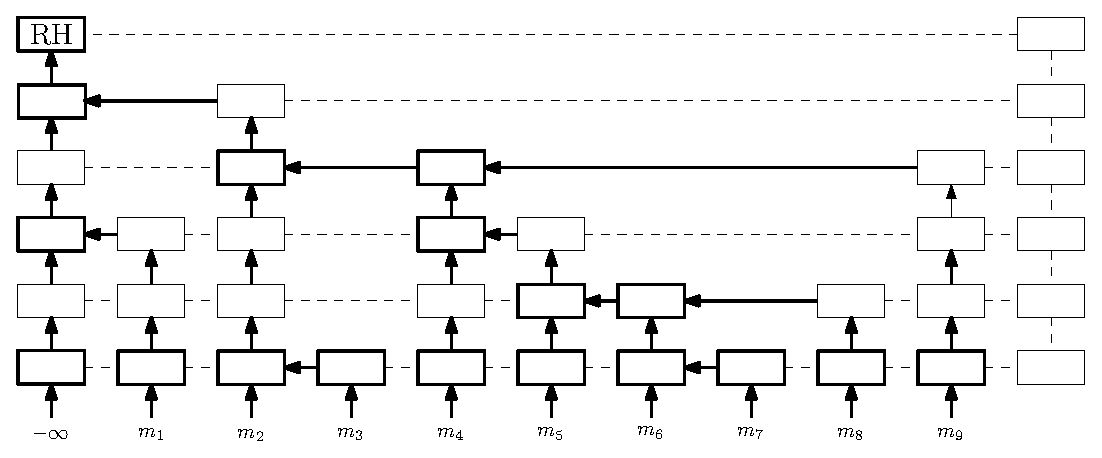
\includegraphics[scale=0.6]{figure/hashFlow.eps}
			\caption{In alto a sinistra, lo \textit{start node} ha il root hash. $ RH $, dipendente dai valori $ m_{n} $ e dal loro ordinamento sulla baselist.}\label{fig:6}
		\end{figure}
	
		\subsubsection{Operazioni}
		
%			Sezione analoga a quella sulla skiplist semplice. Ovviamente questa è sempre una parte di analisi pertanto le varie spiegazione saranno puramente concettuali,
%			algoritmiche e legate a formule, e non comprenderanno scelte di progettazione.

			In quanto ADS, la skip list autenticata offrirà due tipologie di operazione:
			
			\begin{itemize}
				\item \textbf{Update}, ovvero la possibilità di fare inserimenti o cancellazioni.
				\item \textbf{Query}, con la possibilità di ottenere un valore e verificare la sua integrità.
			\end{itemize}
			
	\subsubsection{Update}
	
%		In questa parte si parla della principale operazione di questa struttura, in funzione proprio dell'utilizzo che se ne fa
%		{Citazione del protocollo}

		{AGGIUNGERE CITAZIONE PROTOCOLLO E TESI GIANMARIA}

		In base a quanto osservabile dai casi d'uso, l'\textit{update} è l'operazione di primaria importanza. Nel momento in cui si vuole modificare, aggiungere o cancellare un valore nello \textit{storage}, la skip list autenticata deve aggiornarsi internamente, proprio a causa di questa modifica. Questo è possibile tramite l'operazione di update. Il client dunque, interagento con la struttura, dovrà specificare il tipo di operazione da svolgere (modifica, aggiunta o cancellazione) e la chiave corrispondente a quel valore.. 
		A seguito dell'invocazione di questa operazione sull'ADS, i valori di hash dei singoli nodi devono essere aggiornati per riflettere il cambiamento che è avvenuto, e con essi il \textit{root hash}.
		Nel caso di inserimento o cancellazione, la prima parte di esecuzione dell'operazione è identica a quella di una skip list semplice, con l'ovvia precisazione che i movimenti avverranno non più sui valori, ma sulle chiavi. Successivamente all'aggiunta/cancellazione del nodo interessato, viene utilizzata la pila precedentemente costituita per aggiornare gli hash dei nodi. Saranno infatti solamente i nodi presenti nella pila, ed eventualmente i suoi vicini di destra, grazie allo schema di hashing precedentemente presentato, a dover essere aggiornati. Pertanto ripercorrendo a ritroso tramite operazioni di \textit{pop} la pila, la struttura dovrà ricalcolare le varie $ f(v) $ di questi nodi e nel caso di inserimento, dei nodi costituenti la nuova torre.
		L'aggiunta in termini di costo computazionale dovuta a questa ulteriore operazione di aggiornamento degli hash, è proporzionale al numero di elementi presenti nella pila. Con alta probabilità l'operazione sarà eseguita in $\mathcal{O}(log{}n)$.
		
		[IMMAGINE CON DUE SKIPLIST PICCOLE AFFIANCATE IN CUI SI EVIDENZIA UN UPDATE DI MODIFICA CON FLUSSI]
					
	\subsection{Proof}
		
%		In questa sottosezione si parla del concetto di Proof, sia da un punto di vista concettuale, sottolineando la sua utilità
%		e riallacciandosi a ciò che è stato detto in parti precedenti, sia da un punto di vista pratico. La parte implementativa con
%		le varie scelte sarà affrontata nel capitolo dedicato al Progetto.
%		{Anche qui supporto di citazione del protocollo}

		{AGGIUNGERE CITAZIONE PROTOCOLLO E TESI GIANMARIA}

		Prima di analizzare l'operazione di query, è necessario soffermarsi sul concetto di \textit{proof}, sopra solo accennato. La proof non è altro che un insieme di \textit{step} da percorrere, secondo un preciso schema che rispecchia lo schema di hashing presente nella struttura dati autenticata, per ottenere il \textit{root hash}. Essa è utilizzato per ottenere una prova, appunto, della validità di un particolare elemento restituito da una query. Infatti oltre a ricevere un generico valore $ x $, corrispondente ad una chiave $ k $, il client ottiene anche una \textit{Proof(k)}, e potrà dunque verificare localmente la corrispondenza tra il proprio root hash locale, \textit{trusted Root Hash}, e quello ottenibile seguendo l'opportuna serie di passi sulla proof ottenuta, \textit{untrusted Root Hash}.
		
	\begin{figure}
		\centering
		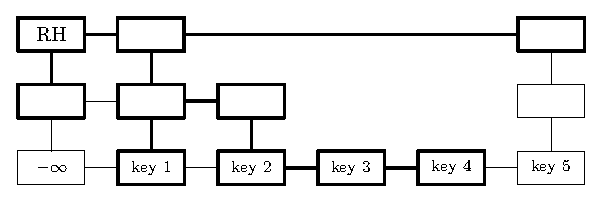
\includegraphics[scale=0.8]{figure/proofExample.eps}
		\caption{\textbf{Esempio di una proof}: i nodi costituenti la proof per la chiave 'key 3' sono evidenziati, così come i collegamenti necessari a ripercorrere gli \textit{step} per ottenere il root hash. Si osservi che la proof sarebbe stata la stessa per la chiave 'key 4' .}\label{fig:9}
	\end{figure}
 		
	\subsection{Query e Verifica}
	
%		Sezione in cui semplicemente si speiga come avviene una query e come è effettuata la verifica tramite la proof precedentemente descritta
%		{Citazione di protocollo}
%		{Schemi}

		{AGGIUNGERE CITAZIONE PROTOCOLLO E TESI GIANMARIA}
	
		Analizzato il concetto di \textit{proof} è possibile ora inserirlo nel più ampio contesto di una query. Un client, a seguito dell'esecuzione di una query su una determinata coppia chiave-valore $ (k,x) $, otterrà una \textit{Proof(k)} relativa a quella chiave. Il client, che memorizza localmente il \textit{root hash} di struttura, ripercorrerà gli \textit{step} opportuni sulla proof, grazie alla conoscenza della particolare funzione crittografica di hash $ h $ correntemente attiva sull'ADS. (Deve cioè effettuare operazioni di hash, nel dato ordine, di tutta una sequenza di hash.) Otterrà dunque il \textit{root hash} presente sul cloud e potrà verificare che questo corrisponda a quello locale. Nel caso in cui questo non accada, vorrà dire che l'integrità del valore ottenuto non è garantita, in quando sono state effettuate delle modifiche sulla struttura, ovvero sul \textit{dataset}. 
			
	
\section{Persistenza}

%	{Analisi prettamente relativa a studio teorico}
%	Qui si inizia a parlare approfonditamente del problema della persistenza approfondendo come si lega all'API. 


